% !TEX root=../MA119-Main.tex


\begin{tcolorbox}[colback=white,colframe=cyan, title filled=false, coltitle=cyan, enhanced, attach boxed title to top center={yshift=-3mm,yshifttext=-1mm}, fonttitle=\bfseries, boxed title style={size=small,colback=white},
title=Logarithmic  function
]
For $x>0$, $b>0$ and $b\neq 1$, we define $y=\log_bx$ to be the number such that $b^y=x$. In other words, 
\[\text{The logarithmic form}\quad y=\log_bx \quad\text{is equivalent to} \quad \text{the exponential form}\quad b^y=x.\] The function $f(x)=\log_bx$ is called  the logarithmic function $f$ of $x$ with the base $b$.

Graphs of logarithmic functions:
\begin{center}
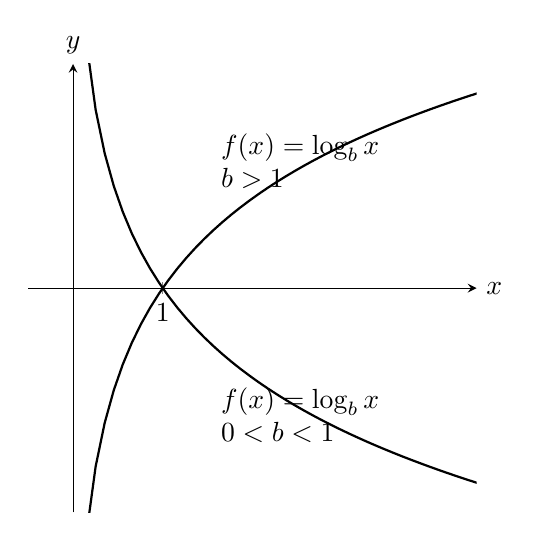
\begin{tikzpicture}
 \begin{axis}[%grid=both, 
 unit vector ratio=1 1,
 xmin=-0.5,xmax=4.5,ymax=2.5,ymin=-2.5, xtick=\empty,ytick=\empty, extra x ticks={1}, 
 axis lines = middle,xlabel=$x$,ylabel=$y$, 
x label style={anchor=west}, y label style={anchor=south}, 
%label style ={at={(ticklabel cs:1.1)}, font={\tiny}}
]
 \addplot[thick, samples=100, y domain=-2.5:2.5]   {ln(x)/ln(2)};
 \addplot[thick, samples=100, y domain=-2.5:2.5]   {-ln(x)/ln(2)};           
\node[anchor=north] at (axis cs:2.75,-1)   {\parbox{2.5cm}{$f(x)=\log_b x$\\ $0< b<1$}};   
\node[anchor=south] at (axis cs:2.75,1)   {\parbox{2.5cm}{$f(x)=\log_bx$\\ $b>1$}};           
  \end{axis}
\end{tikzpicture}
\end{center}
 
\end{tcolorbox}

\begin{tcolorbox}[colback=white,colframe=cyan, title filled=false, coltitle=cyan, enhanced, attach boxed title to top center={yshift=-3mm,yshifttext=-1mm}, fonttitle=\bfseries, boxed title style={size=small,colback=white},
title=Common logarithms and natural logarithms
]
A logarithmic function $f(x)$ with base 10 is called the common logarithmic function and denoted as $f(x)=\log x$.

A logarithmic function $f(x)$ with base the natural number $e$ is called the natural  logarithmic function and denoted as $f(x)=\ln x$.
\end{tcolorbox}


\begin{tcolorbox}[colback=white,colframe=cyan, title filled=false, coltitle=cyan, enhanced, attach boxed title to top center={yshift=-3mm,yshifttext=-1mm}, fonttitle=\bfseries, boxed title style={size=small,colback=white},
title=Basic properties of logarithms
]
 For $b>0$ and $b\neq 1$,
\begin{enumerate}
\item $b^{\log_bx}=x$. 
\item $\log_b(b^x)=x$. In particular, $\log_bb=1$ and $\log_b1=0$.
\end{enumerate}
\end{tcolorbox}


\begin{exercise}
Write each equation into equivalent exponential form.\\

\noindent
\begin{enumerate*}[label=(\alph*)~~]
\item  $\log_b25=2$ \hspace{0.35\textwidth}
\item  $y=\log_213$
\end{enumerate*}
\end{exercise}
\vspace{2cm}


\iffalse
\begin{exercise}
Write each equation into equivalent exponential  form.\\

\noindent
\begin{enumerate*}[label=(\alph*)~~]
\item  $\log_37=y$ \hspace{0.35\textwidth}
\item  $3=\log_b64$
\end{enumerate*}
\end{exercise}
\fi


\begin{exercise}
Write each equation into equivalent logarithmic form.\\

\noindent
\begin{enumerate*}[label=(\alph*)~~]
\item  $e^y=9$ \hspace{0.4\textwidth}
\item  $b^3=8$
\end{enumerate*}
\end{exercise}
\vspace{2cm}


\iffalse
\begin{exercise}
Write each equation into equivalent logarithmic form.\\

\noindent
\begin{enumerate*}[label=(\alph*)~~]
\item  $7^x=10$ \hspace{0.4\textwidth}
\item  $b^5=2$
\end{enumerate*}
\end{exercise}
\fi


\begin{exercise}
Evaluate.
\begin{enumerate}[label=(\arabic*)~~,itemsep=1cm]
\item  $\log_24$
\item  $\log_3\sqrt{3}$
\item  $\log_{27}3$
\item  $\log_55$ 
\item  $\log 1$
\item $2^{\log_22.718}$ 
\end{enumerate}
\end{exercise}



\iffalse
\begin{exercise}
Evaluate.
\begin{enumerate}[label=(\arabic*)~~, itemsep=1cm]
\item  $\log_216$
\item  $\log_93$
\item  $\log_{27}3$
\item  $\log 10$ 
\item  $\ln 1$ 
\item $e^{\ln 2}$
\item $\log 10^{\frac13}$
\end{enumerate}
\end{exercise}
\fi



\begin{exercise}Find the domain of the function $f(x)=\log(2-x)$.
\end{exercise}

\vspace{1cm}


\begin{exercise}
Sketch the graph of each function and find its range.\\

\noindent
\begin{enumerate*}[label=\arabic*)~~]
\item $f(x)=\log_3^x$\hspace{0.3\textwidth}
\item $f(x)=\log_{\frac13}^x$
\end{enumerate*}

\noindent
\begin{minipage}{\textwidth}
\begin{minipage}{0.5\textwidth}
\begin{center}
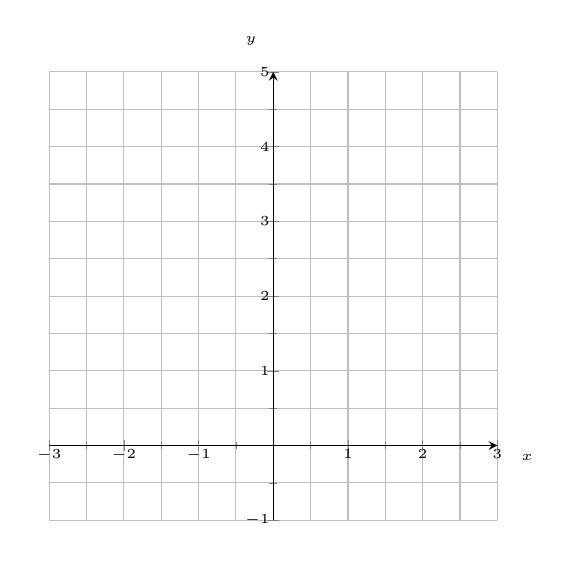
\begin{tikzpicture}
 \begin{axis}[grid=both,unit vector ratio*=1 1, ymin=-1,ymax=5,xmax=3,xmin=-3,xtick={-3,-2,...,3},ytick={-1,0,...,5},minor tick num=1, axis lines = middle,xlabel=$x$,ylabel=$y$, 
x tick label style={yshift=1ex,font={\tiny}}, y tick label style={xshift=1ex, font={\tiny}}, label style ={at={(ticklabel cs:1.1)}, font={\tiny}}
]
 %\addplot[thick, samples=100,domain=1:3.82, name path=A, -stealth]   {(x-2)^2+1};           
 % \addplot[thick, draw] (1, 2)--(-1.95,1.5);
 % \node[draw,shape=circle, minimum size=1.25mm,inner sep=0pt,outer sep=0pt] at (-2,1.5) {};              
  \end{axis}
\end{tikzpicture}
\end{center}
\end{minipage}
\begin{minipage}{0.5\textwidth}

\begin{center}
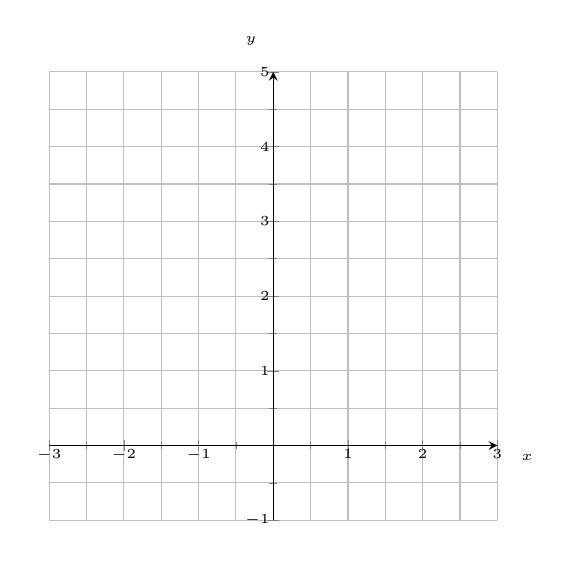
\begin{tikzpicture}
 \begin{axis}[grid=both,unit vector ratio*=1 1, ymin=-1,ymax=5,xmax=3,xmin=-3,xtick={-3,-2,...,3},ytick={-1,0,...,5},minor tick num=1, axis lines = middle,xlabel=$x$,ylabel=$y$, 
x tick label style={yshift=1ex,font={\tiny}}, y tick label style={xshift=1ex, font={\tiny}}, label style ={at={(ticklabel cs:1.1)}, font={\tiny}}
]
 %\addplot[thick, samples=100,domain=1:3.82, name path=A, -stealth]   {(x-2)^2+1};           
 % \addplot[thick, draw] (1, 2)--(-1.95,1.5);
 % \node[draw,shape=circle, minimum size=1.25mm,inner sep=0pt,outer sep=0pt] at (-2,1.5) {};              
  \end{axis}
\end{tikzpicture}
\end{center}
\end{minipage}
\end{minipage}
\end{exercise}



